\documentclass{article}

\usepackage{amsmath,amsfonts,amsthm,amssymb}
\usepackage{fancyhdr}
\usepackage{float}
\usepackage{lastpage}
\usepackage{graphicx}
\usepackage{supertabular}
\usepackage{multirow}
\usepackage{ifthen}
\usepackage{enumerate}
\usepackage{subcaption}
\usepackage[hidelinks]{hyperref}
\usepackage{soul}
\usepackage[mediumspace,mediumqspace,Grey,squaren]{SIunits}

% In case you need to adjust margins:
\topmargin=-0.5in
\evensidemargin=0in
\oddsidemargin=0in
\textwidth=6.5in
\textheight=9.0in
\headsep=0.25in

% Homework Specific Information
\newcommand{\hmwkTitle}{Project Report 3}
\newcommand{\hmwkDueDate}{April 9th, 2014}
\newcommand{\hmwkClass}{42-731}
\newcommand{\hmwkAuthor}{Alex Sun Yoo, Michael Nye, Ozan Iskilibli}
\newcommand{\hmwkEmail}{ayoo, mnye, oiskilib}
\newcommand{\hmwkCollaborators}{}
\newcommand{\bigspace}{\vspace{.25in}}

% Tools for formatting questions
\newcommand{\question}[1] {\vspace{.25in} \hrule\vspace{0.5em}
\noindent{\bf #1} \vspace{0.5em}
\hrule \vspace{.10in}}
\renewcommand{\part}[1] {\vspace{.10in} {\bf (#1)}}

% Setup the header and footer
\pagestyle{fancyplain}
\lhead{\fancyplain{}{\hmwkAuthor \\ \hmwkEmail}}
\chead{\fancyplain{}{\textbf{\hmwkTitle}}}
\rhead{\fancyplain{}{\hmwkClass \\ Due:\ \hmwkDueDate}}
\lfoot{}
\cfoot{}
\rfoot{Page\ \thepage\ of\ \pageref{LastPage}}
\renewcommand\headrulewidth{0.4pt}
\renewcommand\footrulewidth{0.4pt}

% Format paragraphs to have spacing instead of indents
\setlength{\parindent}{0pt}
\setlength{\parskip}{5pt plus 1pt}

% This is used to trace down (pin point) problems
% in latexing a document:
%\tracingall

\renewcommand{\arraystretch}{1.5}

%%%%%%%%%%%%%%%%%%%%%%%%%%%%%%%%%%%%%%%%%%%%%%%%%%%%%%%%%%%%%

\begin{document}

\thispagestyle{plain}
\begin{center}
{\Large \hmwkClass\ \hmwkTitle} \\
\hmwkAuthor \\
\hmwkEmail \\
\ifthenelse{\equal{\hmwkCollaborators}{}}{}{Collaborators: \hmwkCollaborators\\}
Due: \hmwkDueDate\\
\end{center}
%%%%%%%%%%%%%%%%%%%%%%%%%%%%%%%%%%%%%%%%%%%%%%%%%%%%%%%%%%%%%

\section*{Part 1: Microscope Characterization}

\subsection*{B.1 Image Data}

All image data is read into a vector of structs, with consistent field naming. This allows us to write generic functions that can operate on any set of images we pass to it, and gives us a grouping with which to store all results bundled together.


\subsection*{B.2 Characterizing fluorescence image background noise}

To compute noise statistics, we first crop out a region of the image containing noise. To do so, a feature-less region in each image was manually found, and then that region was stored into the script for repeatability. Each image is then cropped using this region, and the mean and variance is calculated over the cropped region. This represents the background region and contains the noise that is analyzed in this section.

To determine the distribution of the data, the noise samples were plotted in a histogram and inspected visually. Upon observation, it was found that the data appears to follow a Gaussian distribution, shown in Figure \ref{fig:noise_dist_background}.

After we observed that the noise followed a Gaussian distribution, we used the Kolmogorov-Smirnov test (implemented in MATLAB as \verb|kstest|) to verify this. This test works by comparing the analytic cumulative distribution function of a distribution to the actually observed CDF for the data. The difference in the distribution gives a confidence interval on how likely the data is to come from a given distribution, and this test confirms with with 95\% confidence that at least 140 of our 150 cropped noise images are drawn from a normal distribution.

To analyze the image sequence over time, we then generated plots showing the mean and variance of the noise over time for the image sequence. We found that both the mean and variance of the noise intensity decreased over time, shown in Figure \ref{fig:noise_mean_var_time}.

To analyze the spatial dependency of the noise, we plotted the mean of noise over columns in one plot, and rows in another (Figure \ref{fig:noise_intensity_space}). We found that the intensity was highest for our noise field in the top left, and lowest in the bottom right. The noise displays a rough linear decay across the image in both the $x$ and $y$ directions.

\begin{figure}[h]
\centering
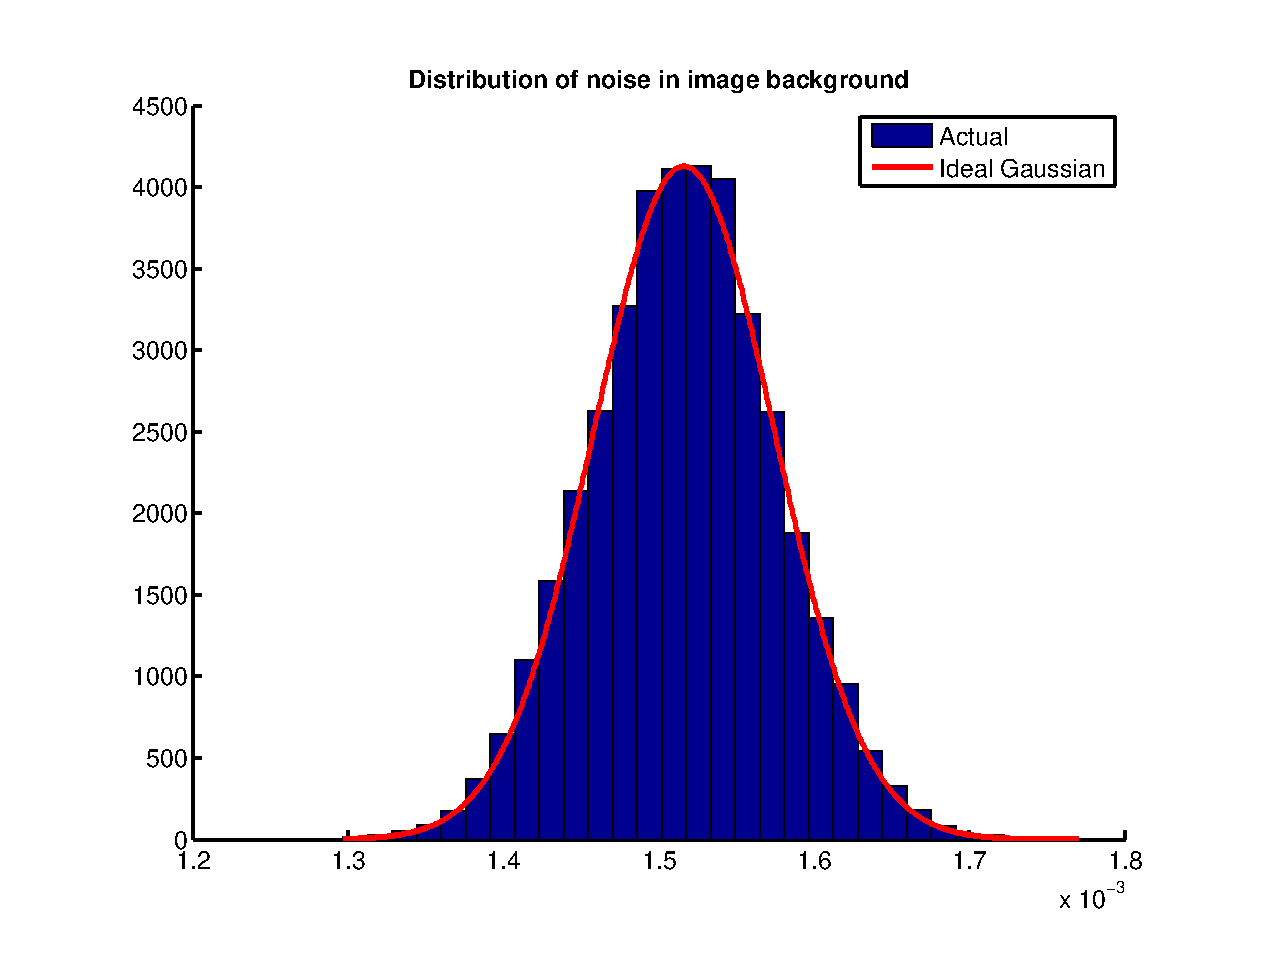
\includegraphics[width=0.7\textwidth]{figures/noise_distribution.pdf}
\caption{Noise distribution in background}
\label{fig:noise_dist_background}
\end{figure}

\begin{figure}[h]
\centering
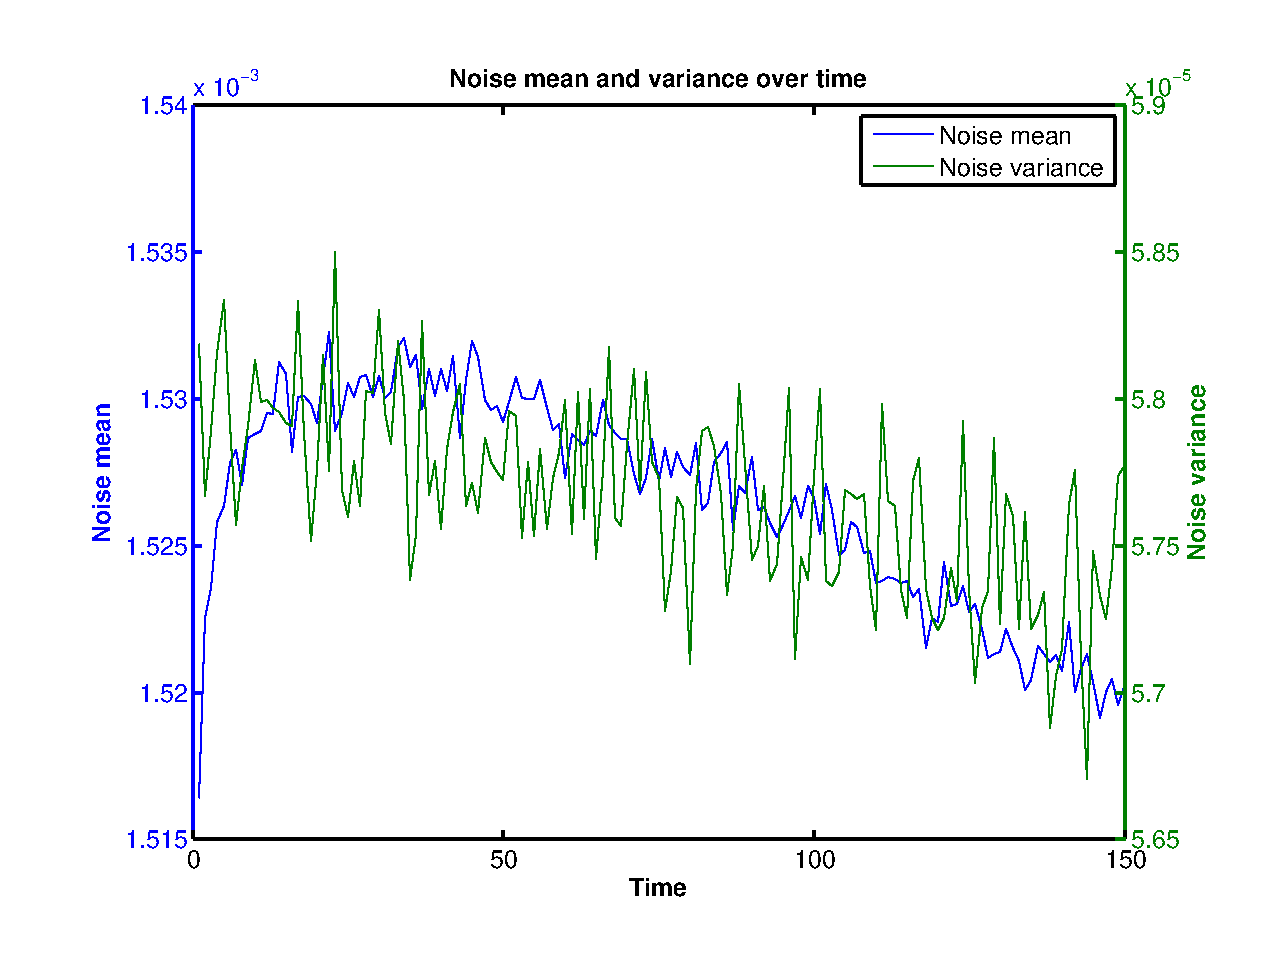
\includegraphics[width=0.7\textwidth]{figures/noise_over_time.pdf}
\caption{Noise Mean \& Variance over time}
\label{fig:noise_mean_var_time}
\end{figure}

\begin{figure}[h]
\centering
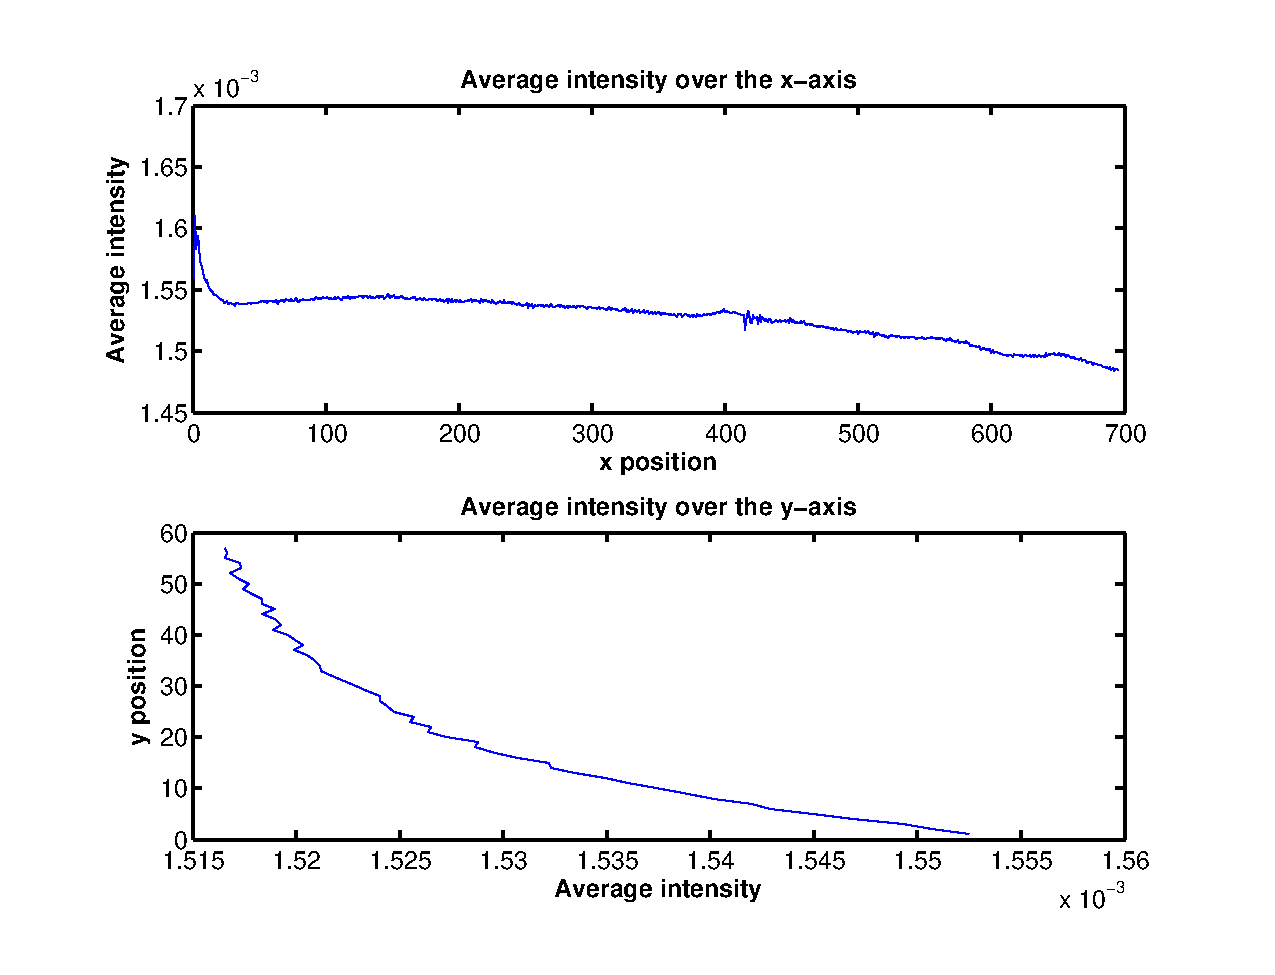
\includegraphics[width=0.7\linewidth]{figures/noise_over_space.pdf}
\caption{Average Noise Intensity over Space}
\label{fig:noise_intensity_space}
\end{figure}


\subsection*{B.3 Characterizing illumination uniformity}

The method \texttt{compuateUniformIllumination} characterizes uniformity of illumination; it accomplishes this by comparing the extrema of the image with how a close-to-ideal uniform image should be. The image is first filtered with a large low-pass Gaussian kernel to smooth out the image; this helps eliminate many extreme outliers that would strongly affect the results.

The global maximum and minimum are then taken from the filtered image and then the difference is found. This difference is compared with the difference of the maximum and minimum of some background noisy image; this is because a background image is an image with close-to-ideal uniformity of illumination, so it is appropriate to compare the two differences. The comparison was selected arbitrarily, and divides the image's extrema difference with the given noise image's extrema difference. The lower and closer to 0 the quotient is, the more uniform the image's illumination is.

The method we used to characterize uniformity of illumination was essentially to compare the extrema of the image with how a close-to-ideal uniform image should be. The image is first filtered with a large low-pass Gaussian kernel to smooth out the image; this helps eliminate many extreme outliers that would strongly affect the results.

The global maximum and minimum are then taken from the filtered image and then the difference is found.  This difference is compared with the difference of the maximum and minimum of some background noisy image; this is because a background image is an image with close-to-ideal uniformity of illumination, so it is appropriate to compare the two differences.

Our characterization method was tested on the first three images, as well as the noisy backgrounds of Images 2 and 3. The calibration noise passed in was the background cropped noise section from Image 1. The results upon running \texttt{computeUniformIllumination} were as follows:

Image 1: 83.1071\\
Image 2: 5.3087\\
Image 3: 5.3079\\
Background Noise 1: 5.0461\\
Background Noise 2: 0.9176\\
Background Noise 3: 0.1283\\

Image 1 has many white portions in it, whereas Images 2 and 3 are much darker overall, when shown on the grayscale image. Thus, Image 1 has worse uniformity than that of Images 2 and 3.\\

\begin{figure}[h]
\centering
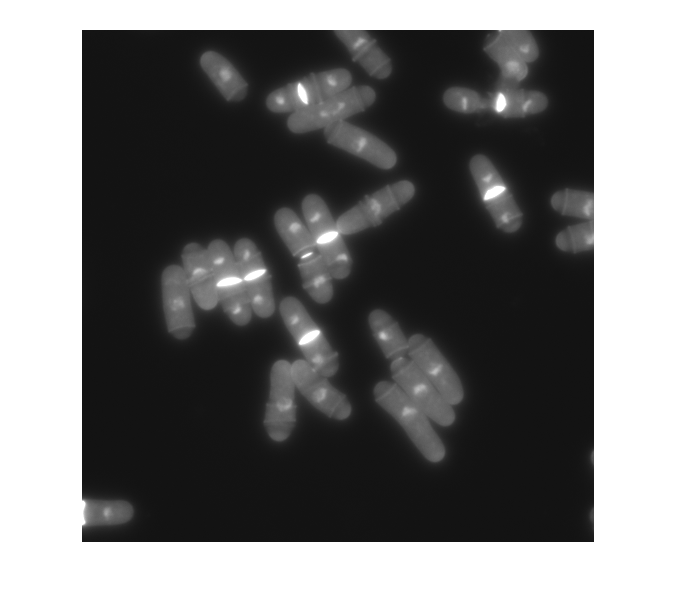
\includegraphics[width=0.3\linewidth]{figures/uniform_illumination_1.png}
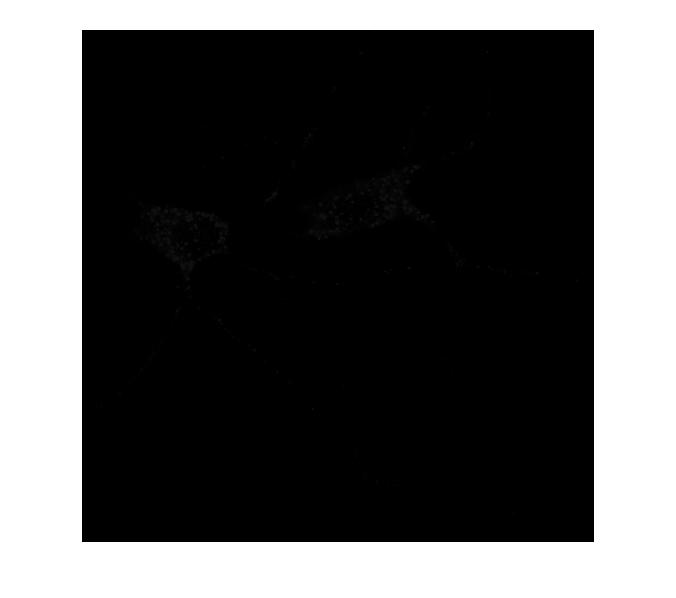
\includegraphics[width=0.3\linewidth]{figures/uniform_illumination_2.png}
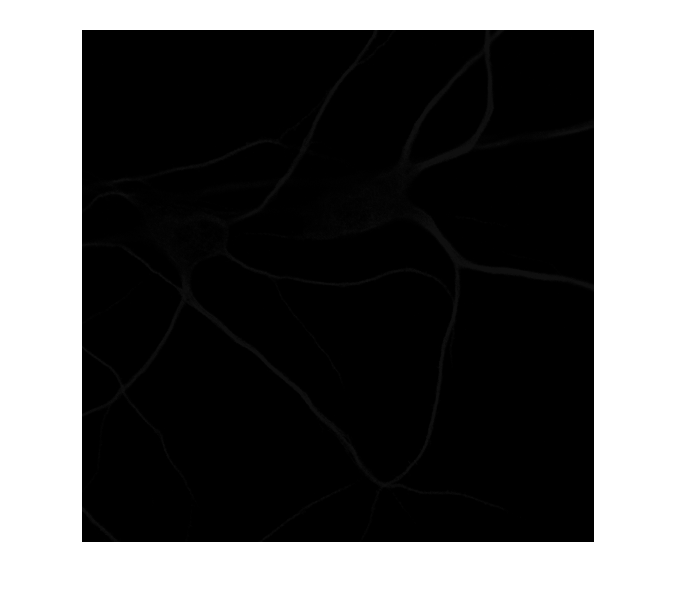
\includegraphics[width=0.3\linewidth]{figures/uniform_illumination_3.png}
\caption{Average Noise Intensity over Space}
\label{fig:illumination_uniformity}
\end{figure}



\subsection*{B.4 Microscope pixel calibration}
 
Two different methods were implemented to calibrate pixel sizes in our images.

The first method is manual. The user is presented with an image, and asked to crop out a section of it along the provided calibration bars. They are then asked to report how many bars wide the section they cropped is. The crop width is then matched with the bar spacing to report the size of each pixel in microns.

The second method is automated. First, the Hough Transform of the image is taken (Figure \ref{fig:houghT}), in the vertical direction, and edges of this transpose are found (Figure \ref{fig:autoCalib}). Once these edges are found, we match the first bar to its neighbor. The distance between these neighbors is taken, and statistical outliers are removed between elements of each bar. Finally, the distance between these bars is used in tandem with the bar spacing to report the size of each pixel in microns. 

The resulting pixel size calculations using each method are given in table \ref{tab:calib}, compared to the actual theoretical pixel size, assuming an optical pixel of \unit{650}{\nano\meter}. The results largely agree with the theoretical calculation, and with each other. The one exception is the 10x zoom level. This automatic calculation is off by a factor of five. This is due to the Hough Transform bar identification. Every fifth bar is taller than the others, so a mis-detection occurs at this small zoom level that leads to an incorrect counting. On the other hand, if this is taken into account, the calibration method calculates a pixel size of \unit{650.5}{\nano\meter} that is only less than 1\% off of the theoretical pixel size at this zoom level. Therefore, the automatic calibration is accepted functioning correctly at this point.

\begin{table}
\caption{Calibration results for different magnification levels and comparison to theoretical pixel sizes}
\label{tab:calib}
\begin{center}
\begin{tabular}{l || r | r || r}
% Caption on top
     Magnification & Manual ($\mu m$) & Automatic ($\mu m$) & Theoretical ($\mu m$) \\
     \hline\hline
     100$\times$                & 63.5            & 62.3               & 65.0 \\ \hline
     60$\times$                 & 107.0           & 115.0              & 108.3 \\ \hline
     20$\times$                 & 325.7           & 344.1              & 325.0 \\ \hline
     10$\times$                 & 641.0           & 130.1              & 650.0 
\end{tabular}
\end{center}
\end{table}



\begin{figure}
\centering
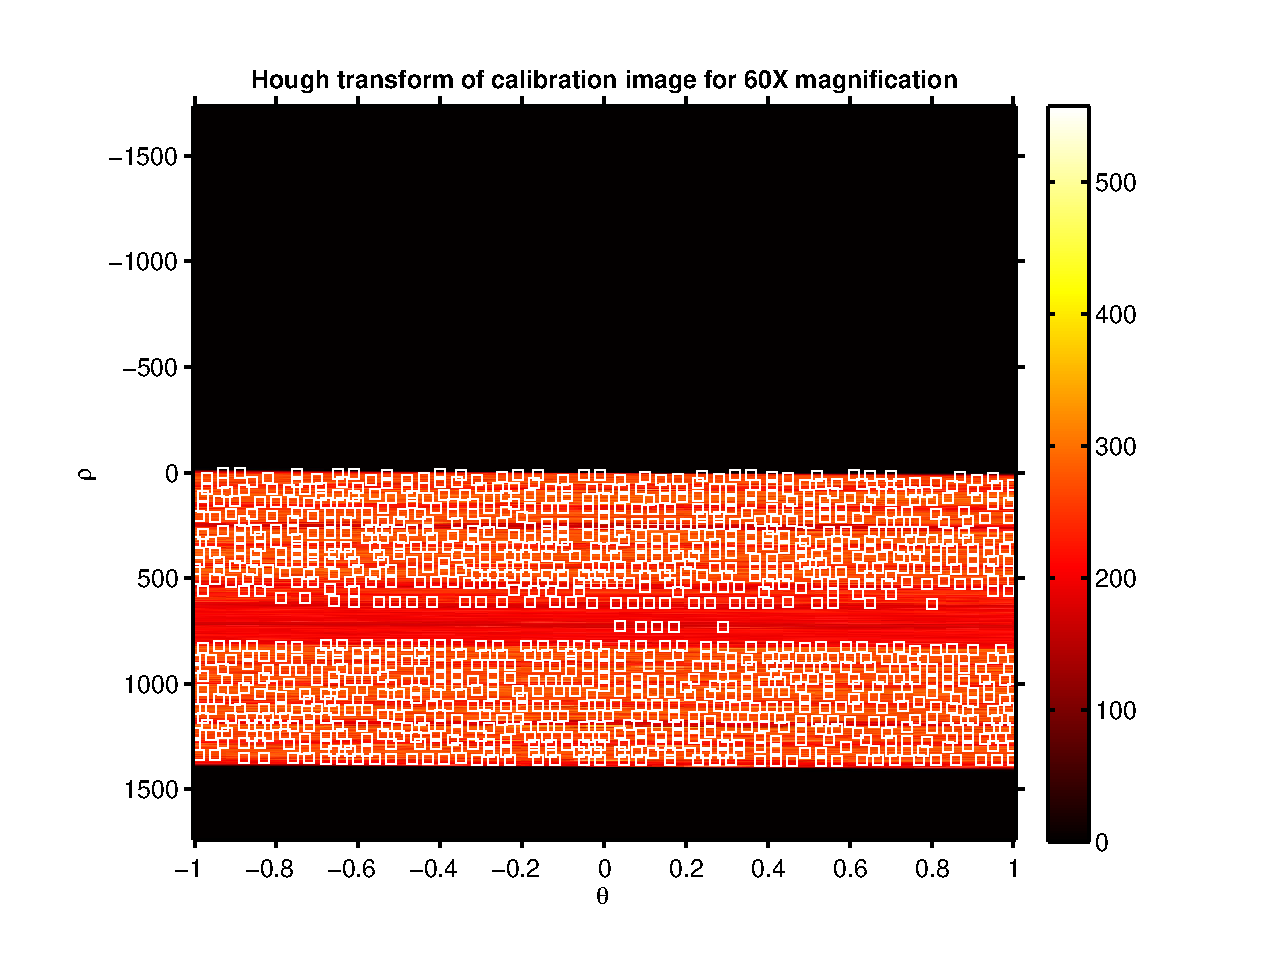
\includegraphics[width=0.75\linewidth]{figures/houghTrans.pdf}
\caption{Hough Transform of the 60$\times$ zoomed in calibration image. The only outcome of this illustration is that the hot spots (white squares) correspond to the $(\theta, \rho)$ pairs of the detected edges. These hot spots are then transformed back into 2D image domain to point out detected edges.}
\label{fig:houghT}
\end{figure}

\begin{figure}
\centering
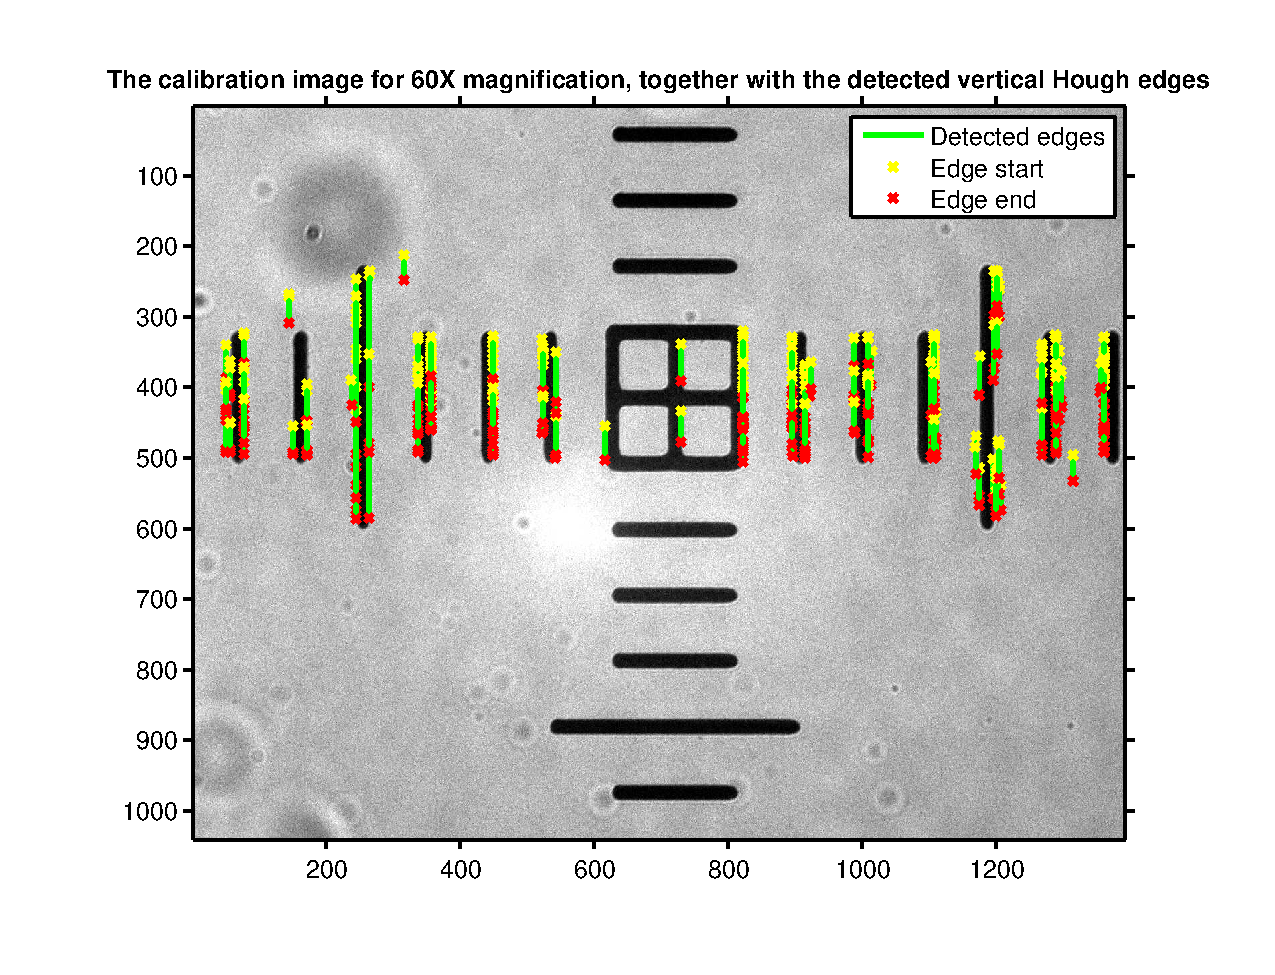
\includegraphics[width=0.75\linewidth]{figures/autocalibration.pdf}
\caption{Detected edges in 60$\times$ zoomed in calibration image using Hough Transform, where green lines show edges, red crosses are edge start points and yellow crosses are edge ends.}
\label{fig:autoCalib}
\end{figure}


\subsection*{B.5 Implementation of a directional anisotropic filter}

In order to detect lines in a certain direction, it can be useful to blur an image more in directions parallel to the line than perpendicular. This can preserve detail in the salient directions while helping to disguise noise off axis. In order to do this, we have implemented a Gaussian anisotropic filter as described by Geusebroek et.\ al.\cite{geusebroek}.

Generating and filtering with 2D anisotropic kernels is simple in theory. However, it is often advantageous to separate a 2D kernel into a composition of two 1D kernels, for decreased computational complexity. This method does that by decomposing an anisotropic Gaussian kernel into a 1D kernel along the x-axis with STD $\sigma_x$, and another 1D kernel along the major axis of the Gaussian with STD $\sigma_\varphi$. Parameters for these kernels are derived as:

\[ a_{11} = \sigma_u^2 \cos^2 \theta + \sigma_v^2 \sin^2 \theta \]
\[ a_{12} = (\sigma_u^2 + \sigma_v^2)\cos\theta \sin\theta \]
\[ a_{22} = \sigma_v^2 \cos^2 \theta + \sigma_u^2 \sin^2 \theta \]
\[ \sigma_x = \sqrt{a_{11} - a_{12}^2/a_{22}} \]
\[ \sigma_\varphi = \sqrt{a_{22}} \]

Our kernels are then convolved with individual rows for the x-axis filter, and then for the interpolated lines at arbitrary pixels along the major axis.

See Figure \ref{fig:anisotropic_filtering} for a sample image filtered at different angles, with $\sigma_u = 10$ and $\sigma_v = 5$. Though it is slightly difficult to see, certain features that are strongly directional are noticeably less distorted in some images than others; for example, at 30\degree vs 120\degree, the center portions of many cells are noticeably thicker.

\begin{figure}[h]
\centering
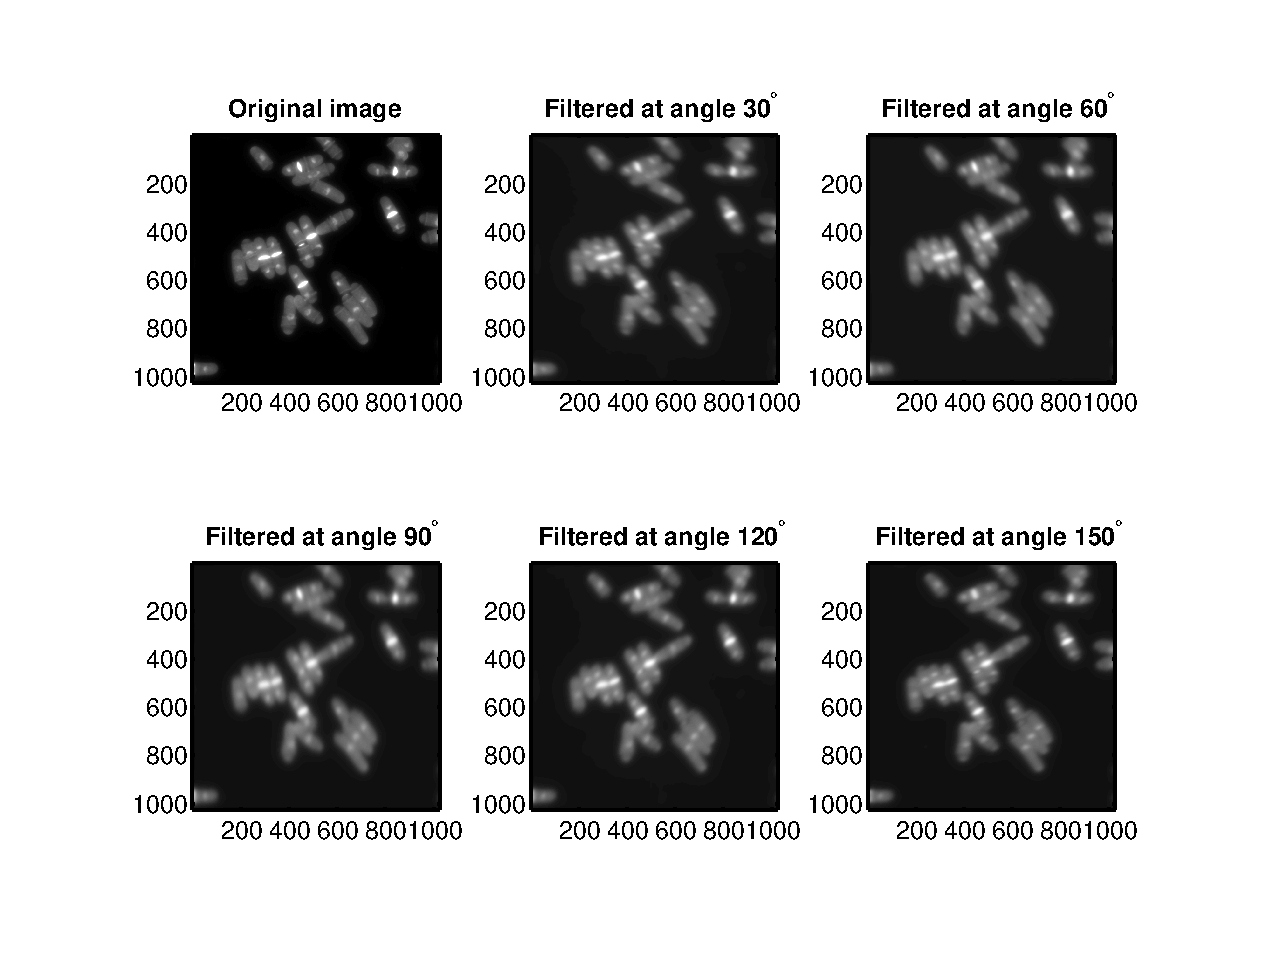
\includegraphics[width=0.95\linewidth]{figures/anisotropic_filtering.pdf}
\caption{Results of filtering with an anisotropic filter at different angles}
\label{fig:anisotropic_filtering}
\end{figure}


\pagebreak
\section*{Part 2: Curvilinear feature detection}

\subsection*{C.1 Implementation of the Steger's algorithm}

We implemented Steger's algorithm to detect and identify pixels on lines and curves of a given image. Our implementation of Steger's algorithm first blurred a given image with a Gaussian kernel with the standard deviation of $\sigma = \frac{n}{\sqrt{3}}$, where $n$ is the estimated maximum line size in pixels. We used $n = 10$ pixels, found by visual estimation on the source images. The MATLAB command \texttt{fspecial} was used to create the Gaussian kernel, followed by \texttt{filter2} for the actual filtering of the image.

Next, both the first and second order partial derivatives are calculated across the entire image in each dimension by taking the differences between the pixels, using \texttt{diff}. The resulting matrices were padded appropriately to match with the iteration through every pixel that will happen for the computational section.

The algorithm then iterates through every pixel in the original image. For each pixel, it creates a Hessian matrix and gradient vector using the precomputed partials. From the Hessian matrix, the eigenvector with the corresponding eigenvalue of greatest magnitude was taken as the direction.

\begin{equation}
\text{direction vector} = [n_x, n_y]
\label{eq:direction}
\end{equation}

The first and second order directional derivatives are then calculated using equations \ref{eq:1_directional_derivative} and \ref{eq:2_directional_derivative}. The location of the local intensity maximum is calculated via equation \ref{eq:local_intensity_max}, then is tested if its magnitude is less than $\frac{1}{2}$. If it is, then the pixel is marked as a center line point.

Results can be found in Figure \ref{fig:line_detect}.

\begin{equation}
r' = [n_x,n_y][f_x,f_y]^T
\label{eq:1_directional_derivative}
\end{equation}
\begin{equation}
r'' = [n_x,n_y]H[n_x,n_y]^T
\label{eq:2_directional_derivative}
\end{equation}
\begin{equation}
x^* = -\frac{r'}{r''}
\label{eq:local_intensity_max}
\end{equation}

\begin{figure}[h]
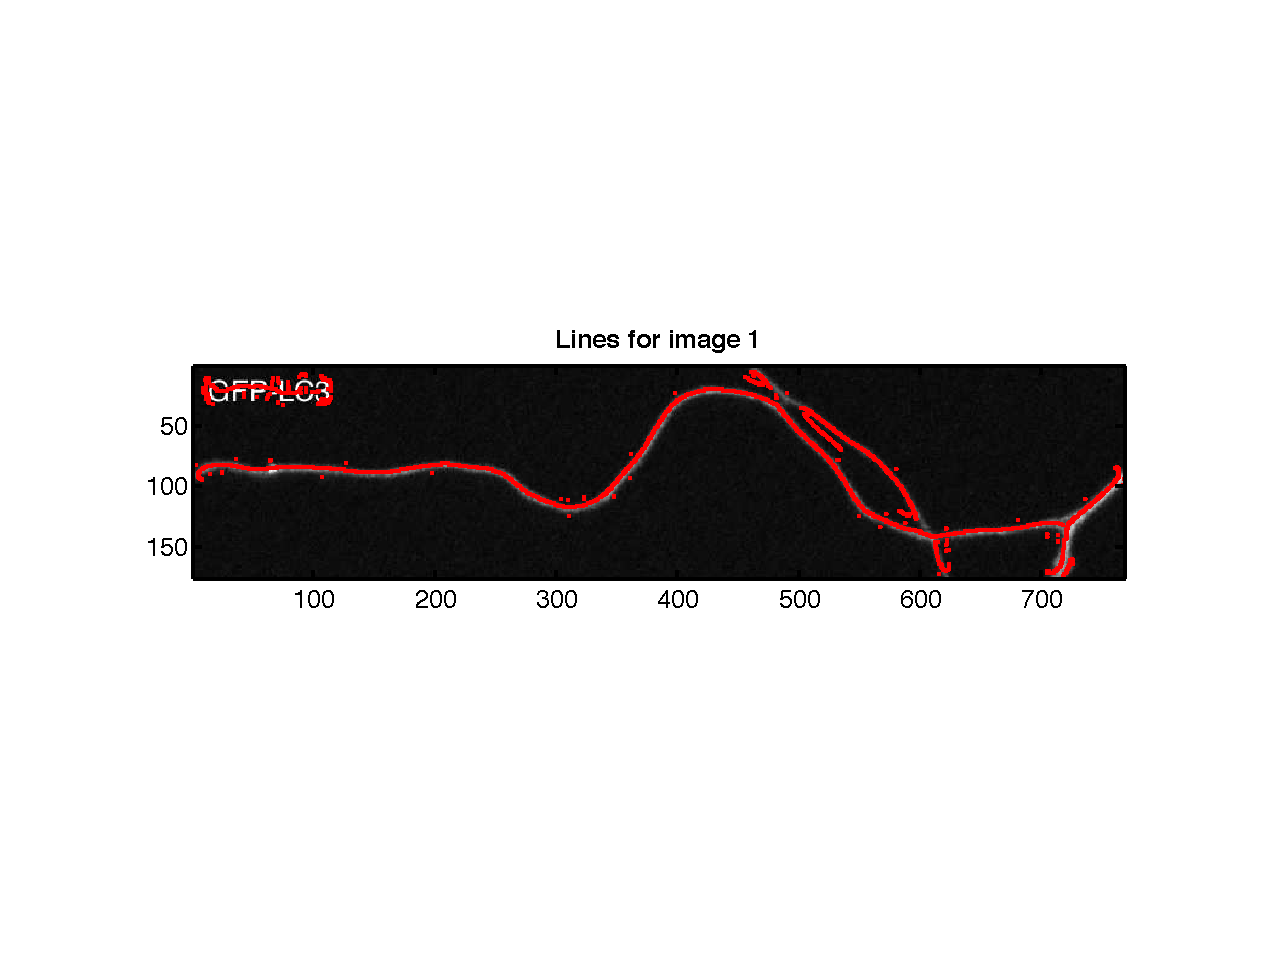
\includegraphics[width=\textwidth]{figures/line_detection_1.pdf}
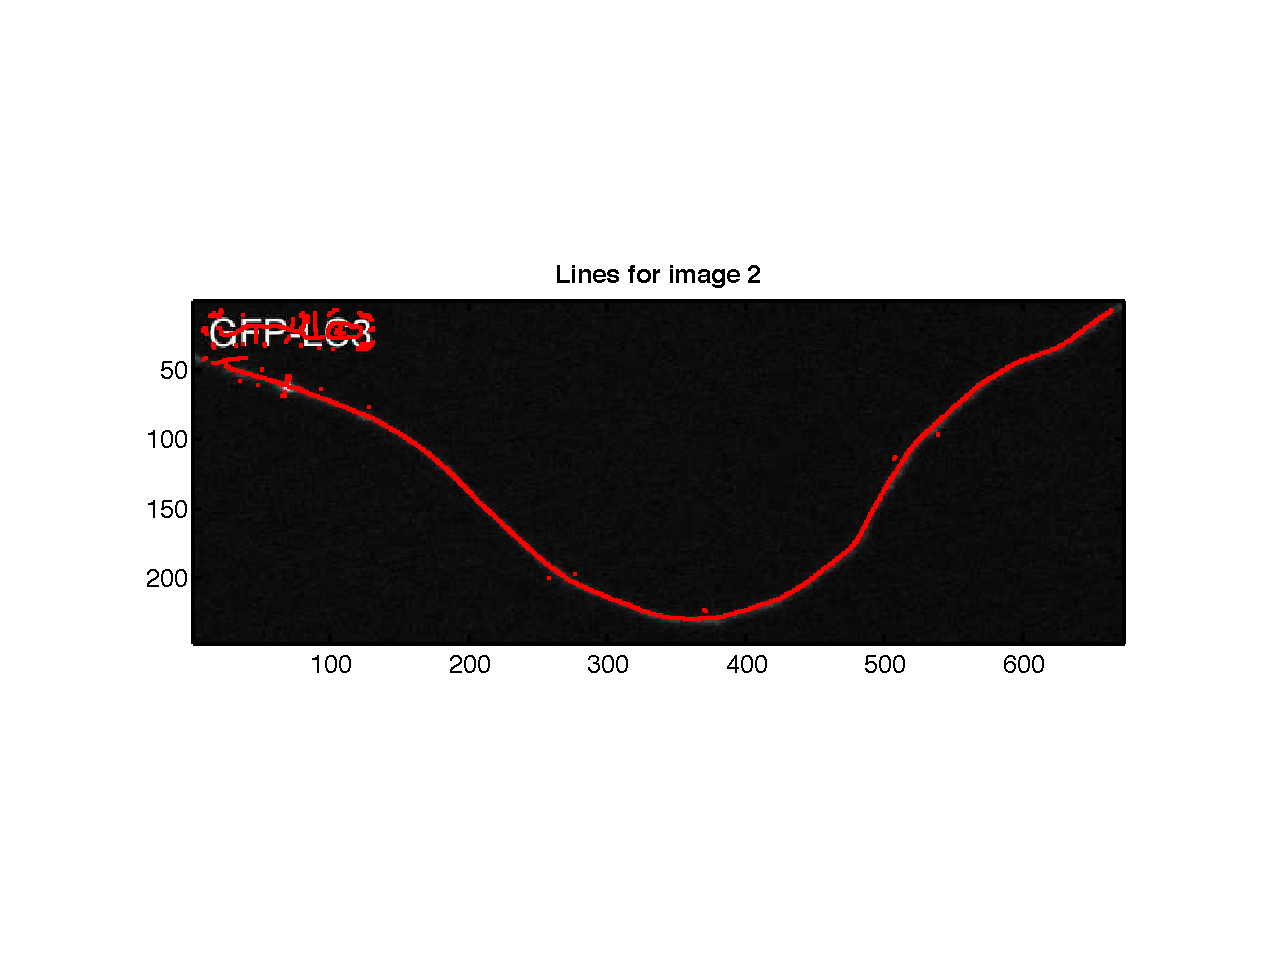
\includegraphics[width=\textwidth]{figures/line_detection_2.pdf}
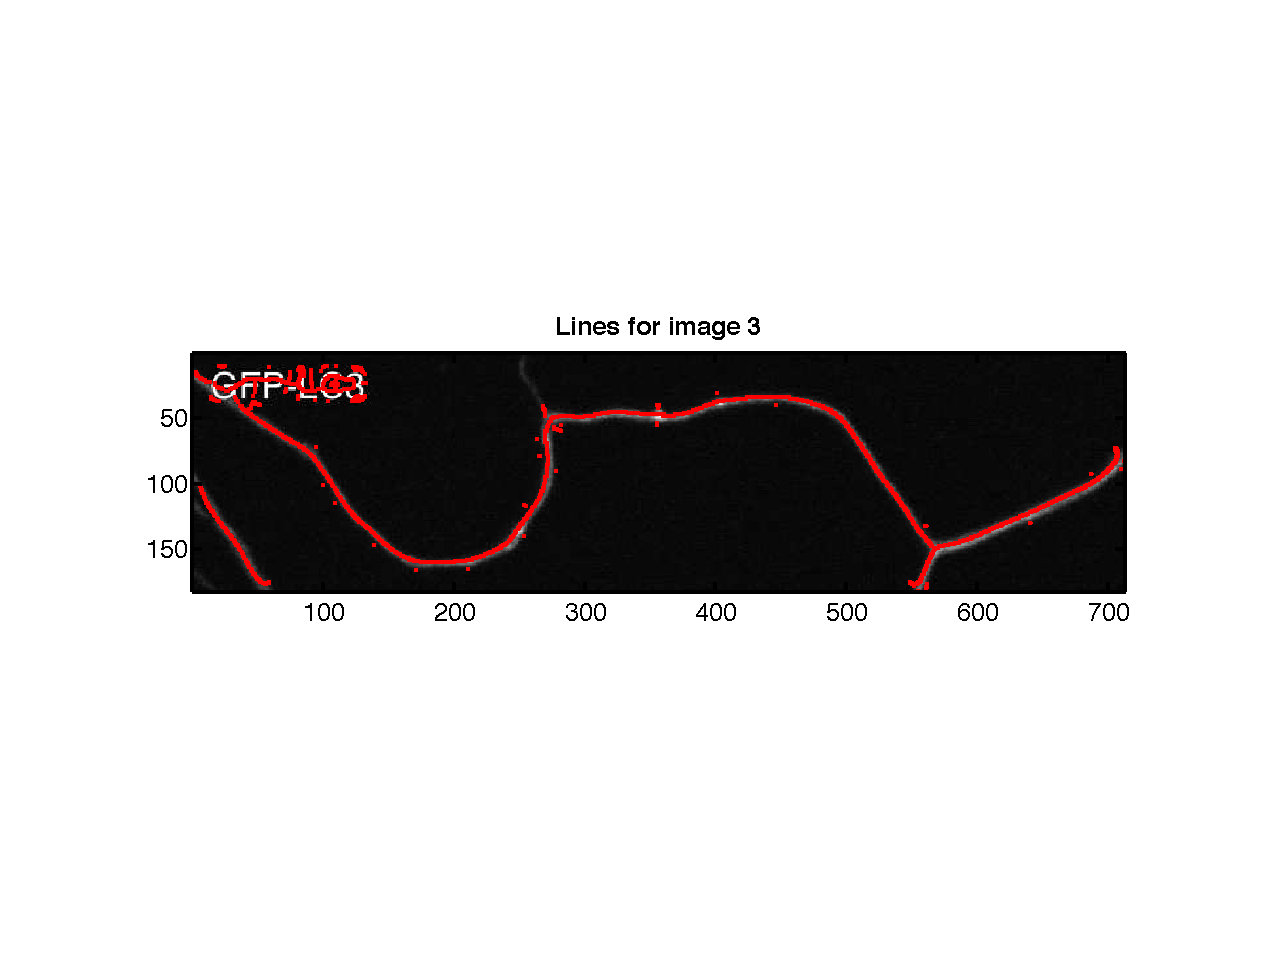
\includegraphics[width=\textwidth]{figures/line_detection_3.pdf}
\caption{Line Detection}
\label{fig:line_detect}
\end{figure}


\subsection*{C.2 Implementation of the pixel Linking operation}

In order to link line pixels together, we begin by sorting the pixels in order of their second directional derivative.

For each pixel, we take its maximal direction, previously computed in C.1 via eigenvector. Once we have this direction, we search out one pixel, checking the three pixels that are closest to the given direction. If a line pixel is found in that direction, then it is added to the line. Search continues in this manner until we find no pixels in the given direction.

We then returned to the original pixel and repeat the above process, but in the opposite direction. Once we have exhausted the other direction, we repeat the overall process at the next pixel in our unsearched set.

If we find a pixel we had already seen, then we consider this a ``junction'', because we have already searched through in a different direction.

Results can be found in Figure \ref{fig:line_linking}.

\begin{figure}[h]
\centering
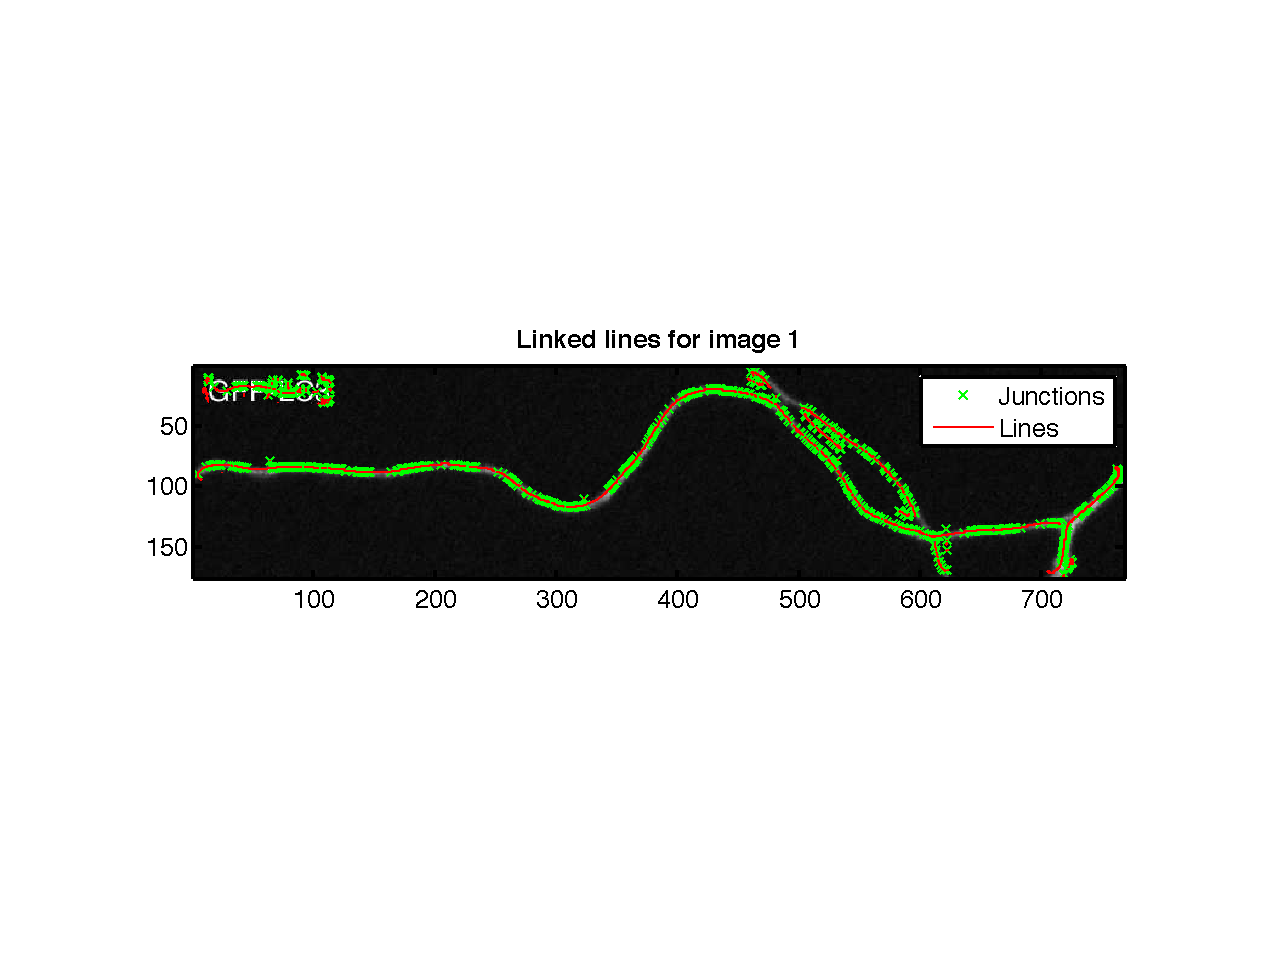
\includegraphics[width=\textwidth]{figures/line_linking_1.pdf}
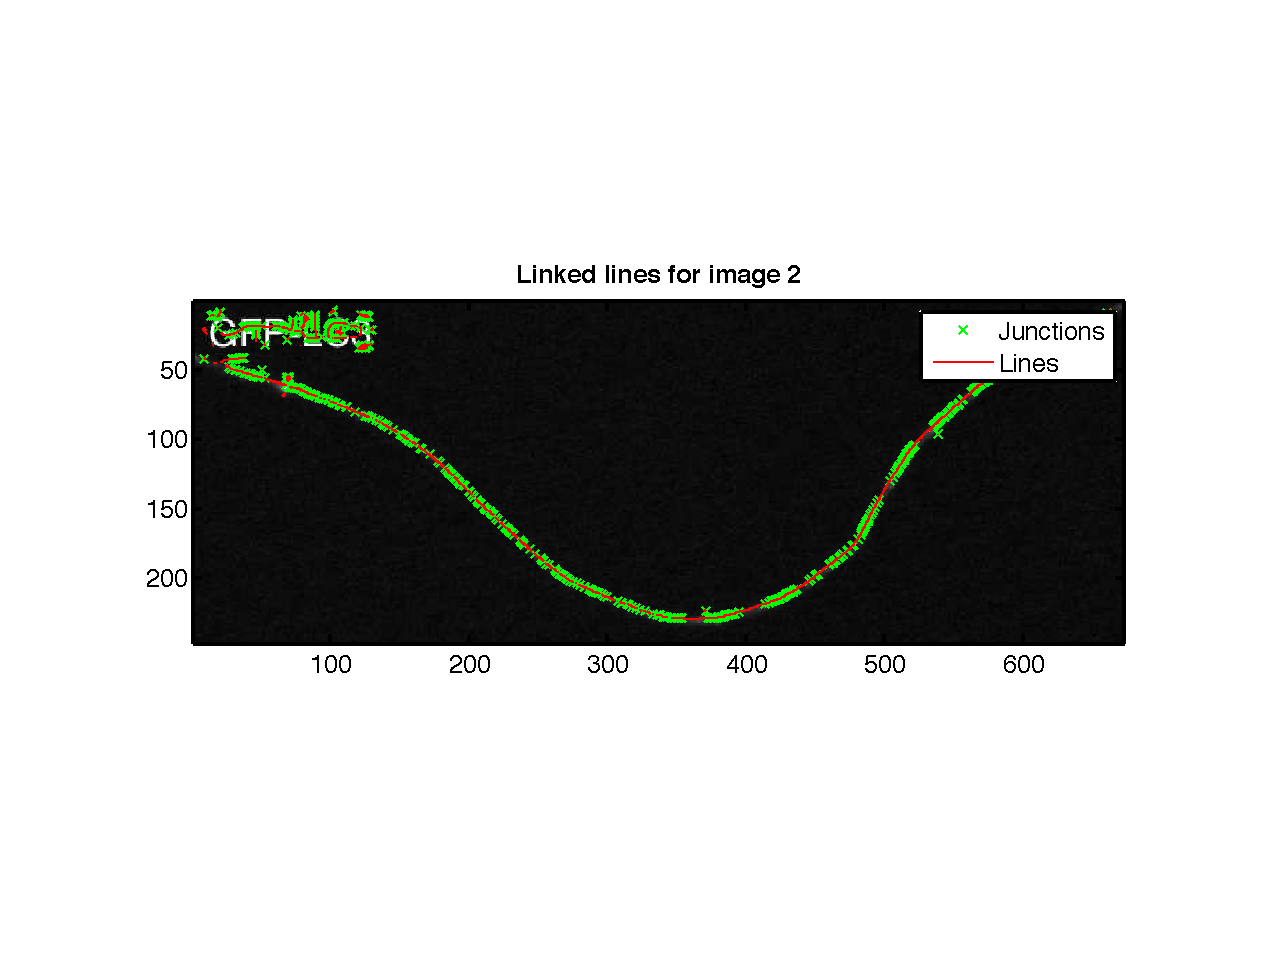
\includegraphics[width=\textwidth]{figures/line_linking_2.pdf}
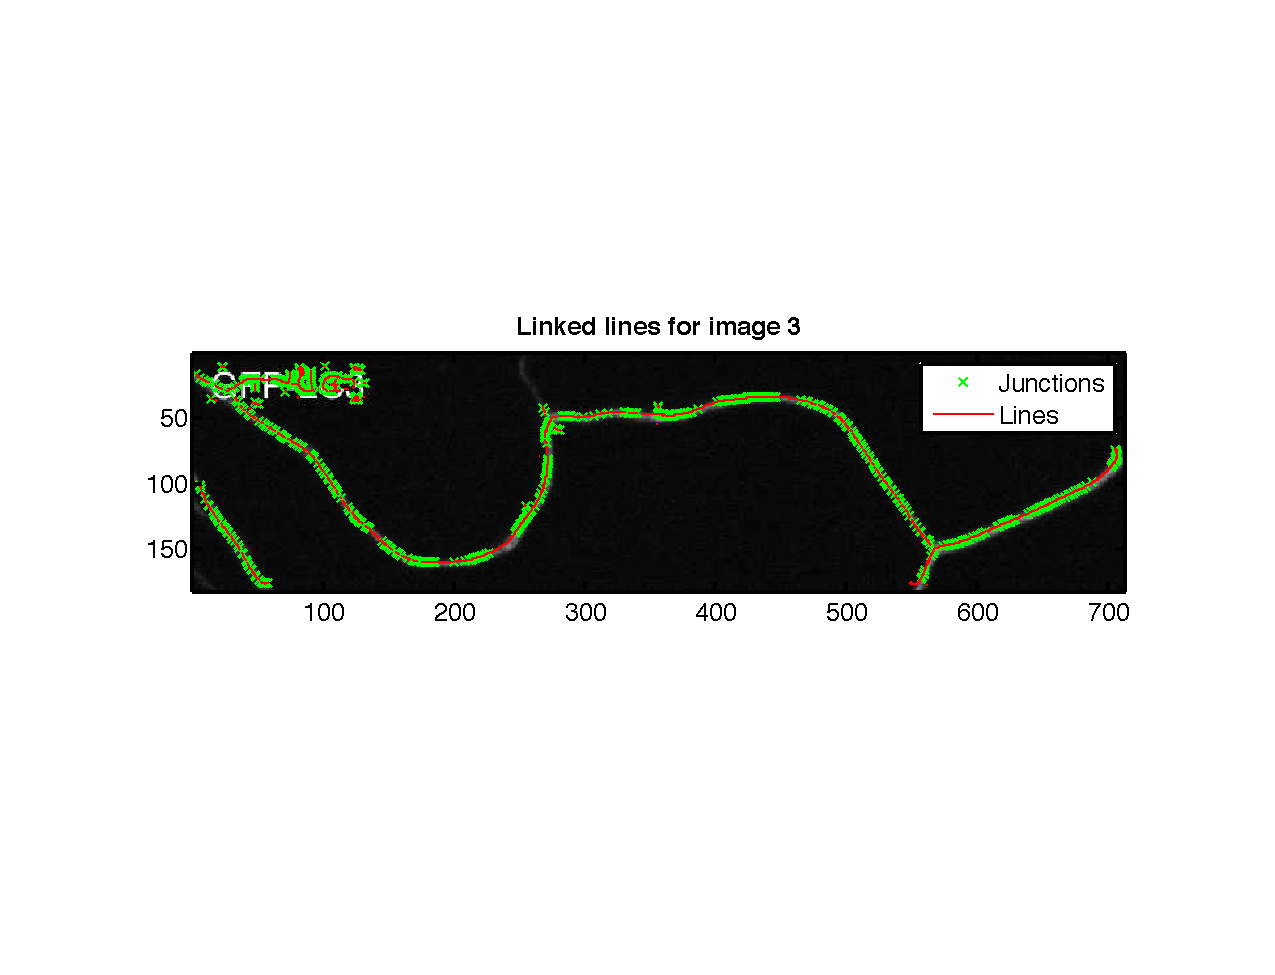
\includegraphics[width=\textwidth]{figures/line_linking_3.pdf}
\caption{Line Linking Results}
\label{fig:line_linking}
\end{figure}



\clearpage
\begin{thebibliography}{9}
\fontsize{10pt}{12pt}\selectfont
\raggedright

    \bibitem{steger}
        C. Steger, An unbiased detector of curvilinear structures, 
        \emph{IEEE Trans. Pattern Analysis and Machine Intelligence},
        vol. 20, pp. 113-125, 1998.

    \bibitem{geusebroek}
        J. M. Geusebroek, A. W. M. Smeulders, and J. van de Weijer, 
        \ul{Fast anisotropic Gaussian filtering},
        \emph{IEEE Trans. Image Processing}, vol. 12, no. 8, pp. 938-943, 2003.


\end{thebibliography}


%%%%%%%%%%%%%%%%%%%%%%%%%%%%%%%%%%%%%%%%%%%%%%%%%%%%%%%%%%%%%

\end{document}

%%%%%%%%%%%%%%%%%%%%%%%%%%%%%%%%%%%%%%%%%%%%%%%%%%%%%%%%%%%%%
